%
%
\comment{

1. The internet is growing --> we need programmable networks ie SDN
2. As a response for this demand, there has been increased adoption of standard APIs to augment current network infrastructures (e.g. OpenFlow)
3. The degree of programmability provided by these APIs are limited by the hardware (data plane)
4. FPGAs bring programmability directly to the hardware; but this comes at a performance and hardware cost
5. NoC-enhanced FPGAs can reduce this cost

\hl{the NoC is a new kind of FPGA interconnect resource that provides pipelining, switching, buffering and stallability. Try to convey this idea. We can use the first few things for latency insensitive/latency-sensitive design. The switching for switch fabrics and on-chip arbitration, the buffering helps in both. This is a very programmable resource and we'll show how best to connect to it, how to use it for different design styles, and how to leverage the NoCs resources in implementing different applications.}

}

Computer networks have seen rapid evolution over the past decade. 
``Cloud computing'' and the ``Internet of Things'' are becoming household terms, as we move to an era where computational power is offloaded from the PC and onto data centers located miles away.
This surge in demand on networking capabilities has led to new network protocols and functionalities being created, updated and enhanced.
The implementation of these protocols and functionalities has proven challenging in current network infrastructures, causing a demand for ``programmable networks''.

Software-Defined Networking (SDN) is a proposed networking paradigm that provides programmability by configuring network hardware (i.e. the ``data plane'') through a separate software-programmable ``control plane''~\cite{nunes2014survey}.
Various APIs have been developed to interface the control plane with the data plane, with OpenFlow~\cite{mckeown2008openflow} being a popular one in the academic community.
However, the degree of programmability provided by these APIs is limited by the capabilities of the hardware contained in the data plane.
If new protocols are developed with functionalities that go beyond what is available in the hardware, then expensive hardware replacements will still be necessary.

Field-programmable gate arrays (FPGAs) have long provided a hardware-programmable alternative to fixed ASIC designs.
The reconfigurability of FPGAs seems like a natural solution to the demand for programmable networks; FPGA designs can be re-programmed in hardware to serve network evolution.
However, what FPGAs gain in programmability they lose in performance; Kuon and Rose quantified the FPGA's programmability overhead to be 18$\times$-35$\times$ in area and 3$\times$-4$\times$ in critical path delay compared to ASICs~\cite{kuon2007measuring}.
As a result, one would expect FPGAs to struggle with efficiently supporting the high bandwidth demands of modern computer networks.

This is generally true; as a whole, established network infrastructures are largely dominated by ASICs.
FPGA designs have made some breakthroughs in various networking applications~\cite{attig2011400,byma2014fpgas,zhou2015packet,muhlbach2010malcobox}, thanks to the increasing transceiver bandwidth available in modern FPGAs (Figure~\ref{txr-bw}).
Despite having these hardened transceivers to bring high bandwidth data onto the chip, these designs still rely on buses made of the FPGA's soft reconfigurable interconnect to move the data across the chip.
These buses are slow (typically 100-400 MHz) and therefore must be made very wide, consuming high amounts of interconnect area and creating challenging timing closure problems for the designer.
Thus, it should come as no surprise that FPGAs have yet to be widely adopted throughout network infrastructures.

%
%\begin{figure}[t] \centering
%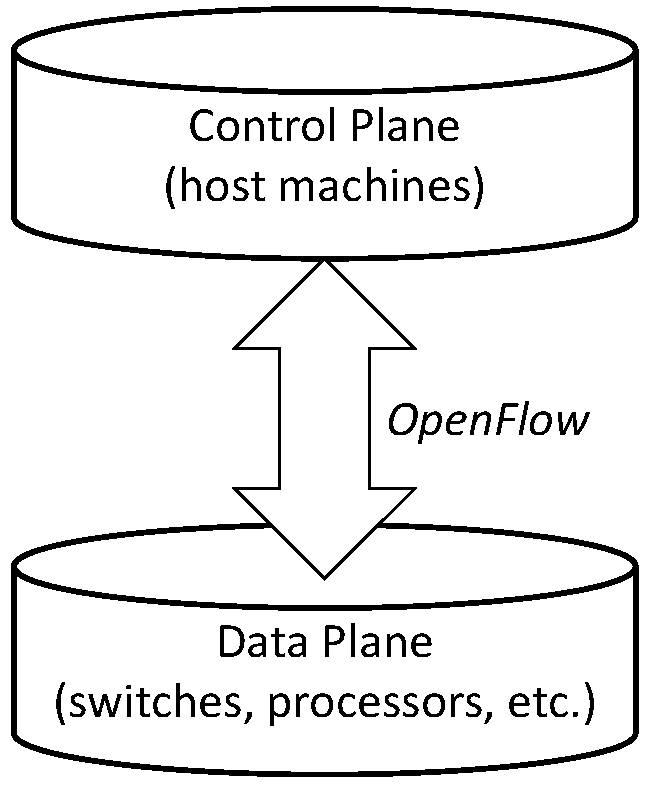
\includegraphics[width=0.25\textwidth]{figs/sdn.pdf}
%\caption{SDN calls for a decoupled control and data plane, with the control plane configuring the data plane hardware through an API such as OpenFlow~\cite{mckeown2008openflow}.}
%\label{sdn}
%\vspace{0cm}
%\end{figure}
%
%
%\begin{figure}[t] \centering
%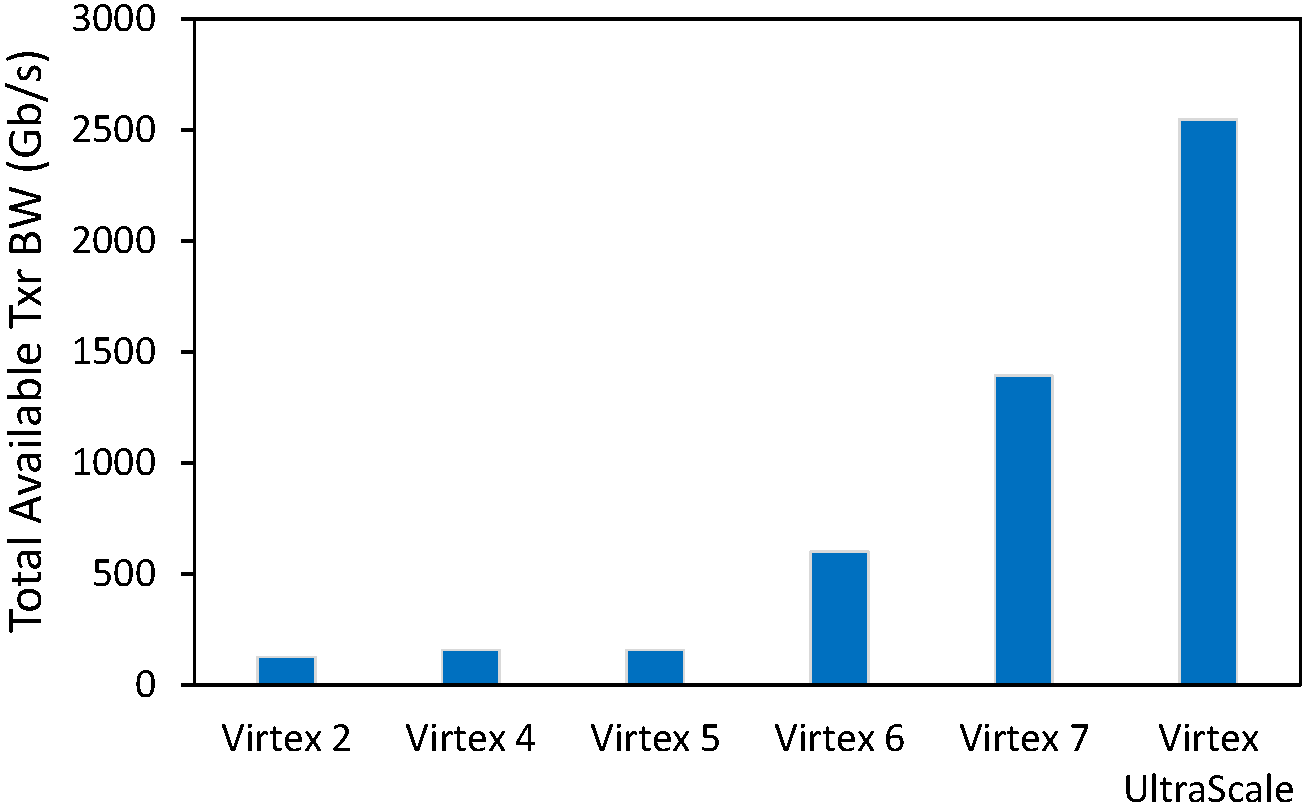
\includegraphics[width=0.4\textwidth]{figs/txr_growth.pdf}
%\caption{Transceiver bandwidth available on Xilinx Virtex devices has rapidly grown with every new generation~\cite{xilds}.}
%\label{fig:txrgrowth}
%\vspace{0cm}
%\end{figure}
%

%
%\figvs{1}{sdn}{}{SDN calls for a decoupled control and data plane, with the control plane configuring the data plane hardware through an API such as OpenFlow~\cite{mckeown2008openflow}.}
%
%
\figvs{1}{txr-bw}{}{Transceiver bandwidth available on Altera Stratix devices has rapidly grown with every new generation. The three data points for each generation correspond to the device models with the three highest transceiver BW.}
%

Recent work has looked closely at this FPGA interconnect problem and has argued for the inclusion of a new system-level interconnect in the form of a Network-on-Chip (NoC)~\cite{abdelfattah2015take}.
Hardening such a NoC in the FPGA's silicon would provide a fast, chip-wide interconnect that consumes a small fraction of the FPGA area~\cite{abdelfattah2015take}.
Such a NoC-enhanced FPGA has the potential to better transport high-bandwidth transceiver data in networking applications.
Prior work has already shown that an efficient and programmable Ethernet switch can be built from a NoC-enhanced FPGA that far outperforms previous FPGA-based switch designs~\cite{bitar2014efficient}.

In this work, we consider another fundamental network building block: the packet processor.
In the most general terms, a packet processor is a device that performs actions based on the contents of received packetized data.
The flexibility of this unit is imperative to the future programmability of computer networks.
Recent works ~\cite{attig2011400,bosshart2013forwarding,gibb2013design,naous2008implementing} have proposed various ways to build packet processors that support SDN/OpenFlow.
The majority base their design on the use of match tables that can be configured to support various types of processing (Section~\ref{sec:bgd}).
Our design takes a different route.
By interconnecting multiple, protocol-specific processing modules through a NoC embedded in an FPGA, we develop a new form of packet processor design that provides a high degree of flexibility for network evolution.
In effect, our design brings programmability directly to the data plane.

Our focus is to explore this new form of packet processor design. To this end, we make the following contributions:

\begin{enumerate}

\item Propose a new packet processor architecture that maximizes hardware flexibility while efficiently supporting modern network bandwidths (400G and 800G).
\item Evaluate the architecture by implementing common packet parsing and processing use-cases.
\item Compare its resource utilization and performance to the best previously proposed FPGA packet processor.
\item Explore how a designer can take advantage of this architecture's flexibility.
%\item Show how the NoC can scale to provide more flexibility and more bandwidth

\end{enumerate}


%
%
